\subsection{Regelbetrieb des ESP}

Zentral bei der Umsetzung des automatisierten Bewässerungssystems ist der ESP32-WROOM-32D Mikrocontroller, welcher die Interaktion zwischen Sensorik, Aktorik und Backend-Systemen steuert. Dabei stellt dieser ESP32 eine umfangreichen GPIO-Ausstattung, welche den Anschluss verschiedenster Peripheriekomponenten ermöglicht.
\\
Im Anschluss an die ESP-Initialisierung, die mittels Wifi-Provisioning sowie Authentifizierung gegen den Backend-Service die Konnektivität sicherstellt, beginnt der zyklische Programmablauf, welcher in verschiedene, klar voneinander getrennte Komponenten untergliedert ist. Diese sind modular aufgebaut und folgen einem Event-Loop-Modell, wie es in Echtzeitbetriebssystemen (RTOS) wie FreeRTOS üblich ist. Die zentrale Steuerung erfolgt durch Tasks, welche Sensorwerte erfassen, verarbeiten, und basierend darauf Aktionen wie etwa die Aktivierung der Pumpe auslösen.
\\
Zur Erfassung der Umweltbedingungen kommen drei Sensoren zum Einsatz: ein \textit{GY-302 BH1750} zur Messung der Beleuchtungsstärke, ein \textit{DHT11}-Sensor zur Ermittlung von Temperatur und Luftfeuchtigkeit sowie ein kapazitiver Bodenfeuchtigkeitssensor (\textit{HiLetgo LM393}). Die Ausgabe der gesammelten Sensordaten erfolgt in periodischen Intervallen über MQTT an eine Solace PubSub Instanz, die über ein Docker-Container-System bereitgestellt wird.
\\
Im Folgenden wird jeder Abschnitt des abstrahierten Ablaufplans des ESP-Regelbetriebs, zu sehen in Abbildung \vref{fig:esp_regelbetrieb}, technisch und funktional erläutert.


\begin{figure}[H]
	\centering
	\vspace{0pt} % verhindert Abstand oben
	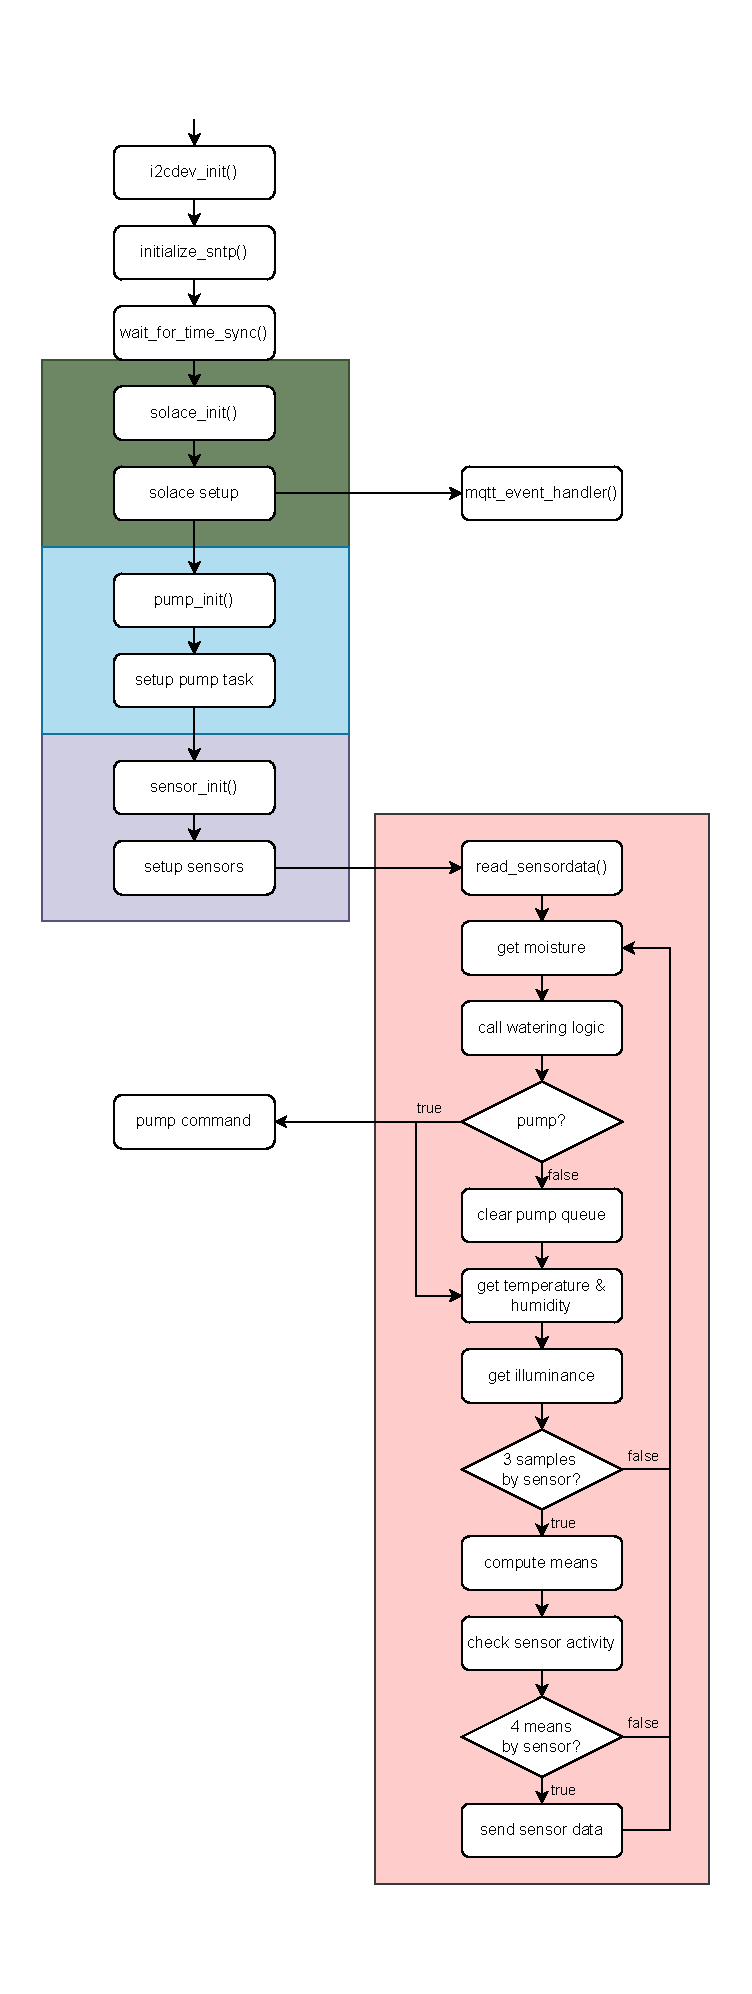
\includegraphics[height=0.97\textheight, keepaspectratio]{./img/esp_regelbetrieb.pdf}
	\caption{Ablaufplan Regelbetrieb des ESP}
	\label{fig:esp_regelbetrieb}
\end{figure}
\newpage

\subsubsection{Systemvorbereitungen: I\textsuperscript{2}C-Stack und Zeitdienst}

Nach Beendigung der initialen Gerätekonfiguration und Abschaltung des Access Points (\texttt{stop\_ap()}) beginnt der ESP32 im Regelbetrieb mit einer Reihe vorbereitender Initialisierungen, die für die korrekte Funktion der Sensorik und Kommunikation essenziell sind. Im Ablaufplan (Abbildung \vref{fig:esp_regelbetrieb}) ist dieser Schritt durch die folgenden Funktionsaufrufe dargestellt:

\begin{itemize}
	\item \texttt{i2cdev\_init()}
	\item \texttt{initialize\_sntp()}
	\item \texttt{wait\_for\_time\_sync()}
\end{itemize}
\vspace{1em}

\noindent Die erste vorbereitende Maßnahme ist die Initialisierung des I\textsuperscript{2}C-Stacks. Die Funktion \texttt{i2cdev\_init()} stammt aus einer externen Bibliothek und abstrahiert die Konfiguration des I\textsuperscript{2}C-Busses, welcher für die Kommunikation mit dem BH1750-Lichtsensor erforderlich ist. Der Sensor wird über die standardisierte I\textsuperscript{2}C-Schnittstelle betrieben und benötigt einen initialisierten Treiberstack, bevor Lese- oder Schreibzugriffe erfolgen können. Im Falle eines Fehlers bei der Initialisierung wird der Systemstart abgebrochen und eine entsprechende Fehlermeldung ausgegeben. Diese Maßnahme dient der Robustheit und stellt sicher, dass keine fehlerhaften Sensordaten erzeugt werden, die zu falschen Bewässerungsentscheidungen führen könnten.
\\
Im Anschluss an die I\textsuperscript{2}C-Vorbereitung erfolgt die Synchronisierung der Systemzeit über das Simple Network Time Protocol (SNTP). Die korrekte Zeit ist essenziell, da alle Sensordaten, die später an das Backend übertragen werden, mit Zeitstempeln versehen werden. Diese Zeitstempel sind wiederum entscheidend für die korrekte Interpretation und Verarbeitung im Backend, insbesondere in Systemen, die auf Zeitreihenanalysen oder historischen Vergleichswerten basieren.
\\
Die Funktion \texttt{initialize\_sntp()} konfiguriert einen SNTP-Client im Polling-Modus und setzt den verwendeten Zeitserver (standardmäßig \texttt{pool.ntp.org}). Anschließend wird in der Funktion \texttt{wait\_for\_time\_sync()} geprüft, ob eine gültige Systemzeit empfangen wurde. Diese Überprüfung erfolgt durch wiederholtes Abfragen der lokalen Zeitinformationen. Der Ablauf ist so gestaltet, dass der ESP32 so lange blockiert, bis eine Zeit verfügbar ist, deren Jahr größer als 2016 ist – dies dient als Heuristik für eine erfolgreiche Synchronisierung.
\\
Diese Zeitsynchronisation ist ein zentrales Qualitätsmerkmal des Systems, da sie nicht nur zur Zeitstempelung der Messwerte dient, sondern auch für die Vergleichbarkeit mit Zielwerten im Backend sowie für langfristige Protokollierungen notwendig ist. Eine falsch synchronisierte Uhr würde beispielsweise zu verzerrten Zeitreihen führen und könnte fehlerhafte Rückschlüsse auf das Verhalten der Pflanzen oder das Klimaregime erlauben.
\\
Insgesamt dienen die beschriebenen Systemvorbereitungen also sowohl der Sicherstellung einer funktionierenden Peripheriekommunikation (über I\textsuperscript{2}C) als auch der korrekten zeitlichen Einordnung aller Mess- und Steuerdaten (über SNTP). Beide Schritte bilden somit eine essenzielle Grundlage für den nachfolgenden zyklischen Ablauf im Regelbetrieb.

\subsubsection{MQTT-Kommunikationsclient}

Nach Abschluss der systemnahen Initialisierungen folgt im Regelbetrieb die Anbindung an die Backend-Infrastruktur über das MQTT-Protokoll. Dies erfolgt durch den Aufruf der Funktion \texttt{solace\_init()}, welche im Ablaufplan (Abbildung \vref{fig:esp_regelbetrieb}) das \enquote{solace setup} sowie den \texttt{mqtt\_event\_handler()} anstößt.
\\
Die MQTT-Kommunikation basiert in diesem System auf dem Publish-Subscribe-Modell und erfolgt über eine Solace PubSub Instanz, welche als Docker-Container bereitgestellt wird. Der ESP32 agiert dabei als Publisher und Subscriber zugleich: Er veröffentlicht periodisch aggregierte Sensordaten und empfängt gleichzeitig neue Zielwerte zur Parametrisierung der Regelstrategie (z.\,B. Soll-Bodenfeuchtigkeitswerte).
\\
Im Rahmen der \texttt{solace\_init()}-Funktion werden zunächst die aus dem nichtflüchtigen Speicher geladenen Verbindungsparameter wie Benutzername, Passwort, Client-ID sowie die spezifischen Topics konfiguriert. Anschließend wird der MQTT-Client initialisiert und mit dem Broker verbunden. Die Verbindung wird dabei so konfiguriert, dass keine Session-Daten zurückgesetzt werden (\texttt{disable\_clean\_session = true}), was eine persistente Kommunikationsbeziehung zwischen Controller und Broker ermöglicht.
\\
Nach erfolgreicher Verbindung registriert der Client einen Event-Handler, der unter anderem auf das Eintreffen neuer Datenpakete reagiert. Ein zentrales Element dieser Kommunikation ist die Funktion \texttt{send\_message()} (zu sehen unter Listing \vref{lst:send_data}), welche zum Versand der aggregierten Sensordaten dient. Diese Funktion nimmt eine bereits als JSON-formatierte Zeichenkette entgegen und überträgt diese mithilfe des MQTT-Clients auf das konfigurierte Topic:
\\

\begin{lstlisting}[style=cstyle, caption={Senden der Sensordaten}, label={lst:send_data}]
	void send_message(const char *message) {
		if (message != NULL) {
			esp_mqtt_client_enqueue(client, info.solace_publish_topic, message, 0, 1, 1, true);
		}
	}
\end{lstlisting}
\vspace{1em}
\noindent Die Nutzung der Funktion \texttt{esp\_mqtt\_client\_enqueue()} ermöglicht dabei eine nicht-blockierende Übertragung, bei der die Nachricht in die interne Queue des MQTT-Stacks geschrieben wird. Durch das Setzen der QoS-Stufe (Quality of Service) auf 1 wird sichergestellt, dass die Nachricht mindestens einmal zuverlässig zugestellt wird – ein angemessener Kompromiss zwischen Zuverlässigkeit und Latenz für diese Anwendungsklasse.
\\
Umgekehrt werden eingehende Steuerinformationen, die z.\,B. neue Zielwerte für Bodenfeuchte, Temperatur oder Beleuchtung enthalten, vom Event-Handler verarbeitet, sobald eine MQTT-Nachricht auf dem Subscription-Topic eintrifft. In diesem Fall wird der Nachrichtenspeicher zunächst allokiert und die empfangenen Daten sicher aus dem Event-Buffer kopiert, wie in folgendem Listing \vref{lst:receive_data} zu sehen ist:
\\

\begin{lstlisting}[style=cstyle, caption={Empfangen von Solace-Daten}, label={lst:receive_data}]
	char *msg = malloc(event->data_len + 1);
	if (msg == NULL) {
		break;
	}
	memcpy(msg, event->data, event->data_len);
	msg[event->data_len] = '\0';
	
	process_received_json(msg);
	
	free(msg);
\end{lstlisting}
\vspace{1em}
\noindent Die manuelle Speicherverwaltung (Allokation und Freigabe) stellt sicher, dass keine Datenverluste auftreten, wenn mehrere MQTT-Ereignisse in schneller Folge eintreffen. Der Zwischenschritt über \texttt{memcpy()} ist notwendig, da der Zeiger \texttt{event->data} nur innerhalb des Event-Kontexts gültig ist. Nach dem Kopieren wird der Inhalt an die Funktion \texttt{process\_received\_json()} übergeben, welche das JSON-Objekt parst und die enthaltenen Zielwerte in den persistenten Flash-Speicher schreibt. Dadurch werden Sollwerte zur Laufzeit aktualisiert und unmittelbar im weiteren Sensorzyklus wirksam.
\\
Insgesamt übernimmt die MQTT-Client-Initialisierung eine zentrale Rolle im System, da sie die bidirektionale Kommunikation zwischen Hardware-Controller und Backend sicherstellt. Sie erlaubt nicht nur die kontinuierliche Datenerfassung und -übermittlung, sondern auch die Fernparametrierung des Systems durch das Backend. Das asynchrone Design mit Event-Handlern, QoS-gestütztem Datentransport und stabiler Speicherverwaltung entspricht den Anforderungen moderner IoT-Anwendungen hinsichtlich Robustheit, Modularität und Echtzeitfähigkeit. \\
Desweiteren wird der verwendete MQTT-Client mit einem automatischen Reconnect-Mechanismus betrieben, um eine hohe Verfügbarkeit der Kommunikation sicherzustellen. Tritt ein Verbindungsabbruch auf, erkennt der zugrunde liegende MQTT-Client der ESP-IDF diesen Fall und übernimmt selbstständig Wiederverbindungsversuche. Dieses Verhalten ist in Echtzeitsystemen mit instabiler oder intermittierender Netzwerkverbindung besonders vorteilhaft, da es die Notwendigkeit eines externen Fehlerbehandlungsmechanismus minimiert und die Robustheit des Systems erhöht. Ein manueller Eingriff durch das Backend ist in solchen Fällen nicht erforderlich.

\subsubsection{Initialisierung der Aktorik (Pumpe)}

Die Initialisierung der Pumpensteuerung erfolgt über die Funktion \texttt{pump\_init()}, welche zwei grundlegende Aufgaben erfüllt: Einerseits wird der für die Relaisansteuerung vorgesehene GPIO-Pin hardwareseitig konfiguriert und initial in einen definierten Zustand versetzt (High = Relais aus), andererseits wird eine dedizierte FreeRTOS-Task mit dem Namen \texttt{pump\_task} gestartet, die in der Abbildung \vref{fig:esp_regelbetrieb} unter \enquote{setup pump task} zu erkennen ist. Diese Task ist dauerhaft aktiv und wartet blockierend auf neue Steuerbefehle, welche durch die Sensorik generiert werden.
\\
Die Pumpe selbst wird über ein SRD-05VDC-SL-C Relaismodul gesteuert, das bei Aktivierung den Stromkreis zur Wasserpumpe schließt. Die Softwarelogik verwendet dazu die \texttt{gpio\_set\_level()}-Funktion, um den Relaiskontakt aktiv (Low) oder inaktiv (High) zu schalten. Eine Initialisierung mit eindeutigem Anfangszustand ist dabei essenziell, um ungewolltes Aktivieren der Pumpe beim Systemstart zu verhindern.
\\
Die Task \texttt{pump\_task} wird über die FreeRTOS-Funktion \texttt{xTaskCreatePinnedToCore()} auf Core 1 des ESP32 platziert. Diese Kernzuweisung erfolgt bewusst, um eine Lastverteilung zwischen Kommunikations- und Sensor-/Aktorlogik zu ermöglichen. Da der WLAN-Stack sowie der MQTT-Client auf Core 0 des ESP32 betrieben werden, ergibt sich durch diese Trennung eine höhere Echtzeitfähigkeit der Pumpenlogik und eine geringere Interferenz zwischen den Tasks. Diese Architekturentscheidung trägt zur Stabilität und deterministischen Ausführung der Aktorik bei, insbesondere unter hoher Netzwerklast. 
\\
Die in Listing \vref{lst:pump_task} gezeigte Erstellung der \texttt{pump\_task} wurde mit einer Priorität von \texttt{5} gewählt, da sie auf eingehende Steuerbefehle schnell und zuverlässig reagieren muss. Die höhere Priorität stellt sicher, dass Pumpvorgänge bevorzugt behandelt werden. Die Stackgröße von \texttt{2048 Bytes} ist ausreichend, da die Task nur einfache Befehle verarbeitet und keine speicherintensiven Operationen durchführt.
\newpage

\begin{lstlisting}[style=cstyle, caption={Start der Pump-Task}, label={lst:pump_task}]
	BaseType_t result = xTaskCreatePinnedToCore(
	pump_task,           // Task-Funktion
	"pump_task",         // Name
	2048,                // Stackgroesse
	NULL,                // Parameter
	5,                   // Prioritaet
	NULL,                // Handle (nicht verwendet)
	1                    // Core 1
	);
\end{lstlisting}
\vspace{1em}
\noindent Neben der Task-Erzeugung wird eine Queue \texttt{pumpQueue} erstellt, welche als asynchrone Kommunikationsschnittstelle zwischen Sensorik und Aktorik dient. Über diese Queue werden Befehle der Struktur \texttt{pump\_params\_t}, welche unter anderem die gewünschte Pumpdauer enthalten, an die Aktorik weitergereicht. Dieses Kommunikationsmuster entspricht dem klassischen \textit{Producer-Consumer-Modell}, bei dem die Sensorik als Ereignisquelle (Producer) fungiert und die Aktorik aufgabenbasiert reagiert (Consumer).
\\
Die Queue dient dabei nicht nur der Synchronisation, sondern ermöglicht auch eine temporäre Entkopplung der Aufgaben. Selbst bei kurzen Verzögerungen in der Ausführung der Pumpen-Task kann ein eingehender Befehl zwischengespeichert werden, was zur Entkopplung der Sensordatenverarbeitung von der physikalischen Ausführung beiträgt. Diese Architekturentscheidung verbessert sowohl die Reaktionsfähigkeit als auch die Systemrobustheit.
\\
Die beiden im Ablaufdiagramm (vgl. Abbildung \vref{fig:esp_regelbetrieb}) aufgeführten Schritte \texttt{pump\_init()} sowie \enquote{setup pump task} stellen also die Grundlage für die Aktorik im Regelbetrieb dar und ermöglichen die automatische Umsetzung von Bewässerungsentscheidungen in hardwareseitige Steuerimpulse.

\subsubsection{Start der Sensorik-Task}

Die kontinuierliche Erfassung und Verarbeitung der Umgebungsdaten bildet das funktionale Zentrum des Regelbetriebs. Dieser Prozess wird durch die FreeRTOS-Task \\
\texttt{read\_sensordata()} realisiert, welche zyklisch die Werte aller verbauten Sensoren erfasst, bewertet, aggregiert und im Anschluss sowohl lokal verarbeitet als auch über MQTT an das Backend übermittelt. Der Start dieser Task erfolgt in der Funktion \texttt{sensor\_init()} und wird explizit dem Core 1 des ESP32 zugewiesen.
\\
Wie auch bei der parallel laufenden Pump-Task, dient die gezielte Platzierung auf Core 1 dazu, Konflikte mit systemnahen Funktionen wie WLAN- und MQTT-Kommunikation zu vermeiden, welche bevorzugt auf Core 0 abgewickelt werden. Durch diese Kerntrennung wird eine deterministische und unterbrechungsarme Ausführung der zyklischen Messprozesse gewährleistet.
\\
Die Erstellung der Task erfolgt mit einer Priorität von \texttt{2} und einer Stackgröße von \texttt{8192 Bytes}. Die moderate Priorität wurde gewählt, da die Sensorik-Task zwar regelmäßig und zuverlässig ausgeführt werden muss, jedoch nicht auf unmittelbare Reaktion angewiesen ist. Eine Priorität von \texttt{2} stellt sicher, dass die Task bei ausreichenden Ressourcen regelmäßig eingeplant wird, jedoch gegenüber zeitkritischeren Prozessen – wie etwa der Pumpensteuerung mit Priorität \texttt{5} – zurücktritt. Diese Priorisierung entspricht den Anforderungen eines Echtzeitsystems, in dem Datenaufnahme zwar zeitnah, jedoch nicht unbedingt unterbrechungsfrei ablaufen muss.
\\
Die vergleichsweise große Stackgröße von \texttt{8192 Bytes} wurde gewählt, um der erhöhten Speicheranforderung durch folgende Faktoren Rechnung zu tragen:
\\
\begin{itemize}
	\item Speicherung mehrerer Sensorwerte und Mittelwerte in Arrays,
	\item Verarbeitung mehrerer \texttt{cJSON}-Objekte bei der MQTT-Nachrichtenerstellung,
	\item Nutzung zusätzlicher Hilfsfunktionen (z.\,B. Zeitstempelerzeugung, Statusprüfung),
	\item Absicherung gegen potenzielle Stacküberläufe bei komplexeren JSON-Strukturen.
\end{itemize}

\vspace{1em}

\begin{lstlisting}[style=cstyle, caption={Start der Sensorik-Task}, label={lst:sensor_task}]
	xTaskCreatePinnedToCore(
	&read_sensordata,     // Task-Funktion
	"read_sensordata",    // Name
	8192,                 // Stackgroesse in Bytes
	NULL,                 // Parameter
	2,                    // Prioritaet
	NULL,                 // Handle (nicht benoetigt)
	1                     // Core-ID
	);
\end{lstlisting}
\vspace{1em}

\noindent Im Ablaufdiagramm (vgl. Abbildung \vref{fig:esp_regelbetrieb}) ist der gesamte Funktionsblock der Sensorik-Task im unteren Bereich dargestellt, beginnend mit dem Schritt \texttt{read\_sensordata()}. Innerhalb der Task werden in einem fortlaufenden Loop nacheinander die Messwerte aller Sensoren erfasst. Dazu zählen:
\\
\begin{itemize}
	\item die Bodenfeuchte über den kapazitiven Sensor (ADC),
	\item Temperatur und Luftfeuchte über den DHT11 (digital, GPIO),
	\item sowie die Beleuchtungsstärke über den BH1750 (I\textsuperscript{2}C).
\end{itemize}
\vspace{1em}

Die dabei gewonnenen Messwerte werden zunächst in Arrays zwischengespeichert. Sobald pro Sensor drei Einzelmessungen (\texttt{SAMPLES = 3}) vorliegen, wird ein arithmetischer Mittelwert gebildet. Dies erfolgt zur Rauschunterdrückung und Glättung von Ausreißern, welche etwa durch Störimpulse oder instabile Umgebungsbedingungen entstehen können. Die entsprechende Funktion \texttt{compute\_mean()}, zu sehen unter Listing \vref{lst:mean}, summiert dazu alle Einzelwerte und berechnet daraus den Durchschnitt. Der Algorithmus ist bewusst einfach gehalten, um Rechenzeit zu sparen und eine konstante Ausführungszeit zu garantieren:
\\

\begin{lstlisting}[style=cstyle, caption={Mittelwertbildung zur Glättung von Sensorwerten}, label={lst:mean}]
	int compute_mean(const int values[]) {
		int sum = 0;
		for (int i = 0; i < SAMPLES; i++) {
			sum += values[i];
		}
		return sum / SAMPLES;
	}
\end{lstlisting}
\vspace{1em}

\noindent Vor der Weiterverarbeitung wird zusätzlich eine Validierung durchgeführt, ob der jeweilige Sensor als aktiv und funktionsfähig eingestuft werden kann. Dabei wird überprüft, ob alle Messwerte innerhalb eines gültigen Wertebereichs liegen. Dies verhindert, dass fehlerhafte Sensoren (z.\,B. durch Kabelbruch oder fehlerhafte Kalibrierung) zu ungültigen Steuerentscheidungen führen. Die Funktion \texttt{is\_sensor\_active()} übernimmt diese Plausibilitätsprüfung:
\\

\begin{lstlisting}[style=cstyle, caption={Überprüfung der Sensoraktivität}, label={lst:sensor_active}]
	bool is_sensor_active(const int values[], int sampleCount) {
		for (int i = 0; i < sampleCount; i++) {
			if (values[i] <= 0 || values[i] >= 4095) {
				return false; // Sensorfehler oder Disconnect
			}
		}
		return true;
	}
\end{lstlisting}
\vspace{1em}

\noindent Sobald vier Mittelwerte (\texttt{MEAN\_COUNT = 4}) pro Sensor vorliegen, erfolgt die Erzeugung einer strukturierten JSON-Nachricht. Diese umfasst Messwerte, Zeitstempel, Sensorstatusinformationen sowie Controller-Metadaten und wird über die zuvor erläuterte Schnittstelle \texttt{send\_message()} via MQTT an das Backend gesendet.
\\
Parallel zur Messwerterfassung wird bei jeder neuen Bodenfeuchte-Messung die Bewässerungslogik aktiviert, wie im Ablaufdiagramm unter \enquote{call watering logic} dargestellt. Die Entscheidungslogik erfolgt durch Aufruf der Funktion \texttt{calculate\_watering\_duration()}, welche im nächsten Abschnitt detailliert beschrieben wird. Führt diese Analyse zu einer positiven Bewässerungsentscheidung, wird ein entsprechender Pump-Befehl über die Funktion \texttt{pump\_send\_command()} an die globale Queue \texttt{pumpQueue} übermittelt, welche als Kommunikationsschnittstelle zur \texttt{pump\_task()} dient und die sichere, asynchrone Übergabe von Steuerbefehlen ermöglicht.
\\
Insgesamt vereint die Sensorik-Task zentrale Aufgaben der Datenerfassung, Signalverarbeitung, Qualitätssicherung, Entscheidungslogik und Backend-Kommunikation. Ihre saubere architektonische Einbindung sowie die klar definierte Schnittstelle zur Aktorik machen sie zu einem robusten und flexiblen Kernbestandteil des Gesamtsystems.

\subsubsection{Bewässerungslogik}

Die Funktion \texttt{calculate\_watering\_duration()} ist für die Ermittlung der notwendigen Bewässerungsdauer auf Basis der Differenz zwischen gemessener und Ziel-Bodenfeuchte zuständig. Sie lädt die Systemkonfiguration, vergleicht Soll- und Ist-Werte und berechnet daraus die Pumpdauer. Um Über- und Unterbewässerung zu vermeiden, wird die Dauer auf definierte Grenzwerte begrenzt.
\\
\\
Die Entscheidung darüber, ob eine Bewässerung erforderlich ist und in welchem Umfang diese erfolgen soll, wird durch die Funktion \texttt{calculate\_watering\_duration()} getroffen. Dieser Funktionsaufruf ist im Ablaufdiagramm unter dem Knoten \enquote{call watering logic} eingezeichnet und bildet das zentrale Bindeglied zwischen der gemessenen Bodenfeuchte und der Ansteuerung der Pumpenlogik.
\\
Die Funktion wird bei jeder neuen Messung der Bodenfeuchte innerhalb der Sensorik-Task aufgerufen. Sie lädt zunächst die gespeicherten Systemdaten, insbesondere den konfigurierten Zielwert für die Bodenfeuchte (\texttt{target\_moisture}) aus dem persistenten Speicher. Anschließend wird geprüft, ob der aktuelle Feuchtewert unterhalb des Sollwertes liegt. Nur wenn ein solches Defizit besteht, wird eine Pumpdauer berechnet.
\\
Wie in Listing \vref{lst:calc_duration} zu erkennen, basiert die Berechnung der Dauer auf einem linearen Modell: Die Differenz zwischen Ziel- und Istwert wird mit einem konstanten Faktor (\texttt{WATERING\_K\_FACTOR}) multipliziert, der in diesem Fall auf \texttt{100} gesetzt wird. Dieses einfache Modell erlaubt eine intuitive Parametrierung und gewährleistet eine proportionale Anpassung der Bewässerungsdauer an das Ausmaß der Trockenheit.
\newpage

\begin{lstlisting}[style=cstyle, caption={Berechnung der Bewässerungsdauer}, label={lst:calc_duration}]
	int calculate_watering_duration(int current_moisture) {
		load_system_data(&info);
		
		if (!info.target_moisture) {
			info.target_moisture = 0;
		}
		
		if (current_moisture >= info.target_moisture) {
			return 0;
		}
		
		int deficit = info.target_moisture - current_moisture;
		int duration = deficit * WATERING_K_FACTOR;
		
		if (duration < MIN_WATERING_TIME) return 0;
		if (duration > MAX_WATERING_TIME) duration = MAX_WATERING_TIME;
		
		return duration;
	}
\end{lstlisting}
\vspace{1em}

\noindent Führt die Funktion zu einer Nicht-Null-Dauer, wird das Ergebnis in Form eines \\\texttt{pump\_params\_t}-Strukturobjekts an die zuvor initialisierte Queue \texttt{pumpQueue} übergeben. Die Übergabe erfolgt über die Funktion \texttt{pump\_send\_command()}, wodurch die asynchron laufende Pumpen-Task (vgl. Listing \vref{lst:pump_task}) aktiviert wird. Dieses Systemdesign gewährleistet eine klare Trennung zwischen Entscheidung und Ausführung, was die Modularität, Wartbarkeit und Reaktionssicherheit des Systems erhöht.
\\
Zusammenfassend bildet die Funktion \texttt{calculate\_watering\_duration()} die Kernkomponente der Regelstrategie. Durch die Kombination aus Zielwertvergleich, linearer Berechnung und Schutzgrenzen wird ein praxisnahes Steuerverhalten realisiert, das zugleich einfach und robust in der Anwendung ist. Ihre Position innerhalb der Sensorik-Task erlaubt eine kontinuierliche Reaktion auf veränderte Umweltbedingungen und macht die Bewässerungsentscheidung zu einem integralen Bestandteil des zyklischen Regelbetriebs.

\subsubsection{Testen der Funktionalitäten}

Die Validierung der im Rahmen dieser Arbeit implementierten Systemfunktionen erfolgte durch eine Kombination aus lokalen Integrationstests und laufzeitbasiertem Debugging über den seriellen Monitor. Ziel war es, sowohl die Korrektheit der Sensorerfassung und Datenverarbeitung als auch die Robustheit der Kommunikations- und Aktorik-Komponenten unter realitätsnahen Bedingungen zu überprüfen.
\\
Ein zentrales Element der Testinfrastruktur war die Verwendung einer containerisierten MQTT-Broker-Umgebung auf Basis von Solace. Der Broker wurde über eine \\\texttt{docker-compose.yml}-Datei lokal bereitgestellt, welche alle relevanten Ports (u.\,a. 1883 für MQTT sowie 8080 für das Web-UI) freigibt und essenzielle Umgebungsparameter für die Broker-Verwaltung definiert. Durch diese Virtualisierung konnte eine vollständig kontrollierte und jederzeit rekonstruierbare Testumgebung geschaffen werden, ohne auf externe Dienste angewiesen zu sein.
\\
Die \texttt{docker-compose.yml} ermöglichte somit die schnelle Inbetriebnahme und erlaubte über das Web-Interface auch die manuelle Kontrolle von Topic-Inhalten, Subskriptionen sowie eingehenden Sensorwerten. Darüber hinaus konnte die Reaktion des Systems auf eingehende Steuerbefehle (z.\,B. Zielwertänderungen) in Echtzeit nachverfolgt und ausgewertet werden. Dieses Setup bildete die Grundlage für systematische Integrationstests der gesamten MQTT-Kommunikationskette.
\\
Zur Laufzeitanalyse des embedded Systems wurde intensiv der serielle Monitor (UART-Konsole) genutzt. Über die im Code implementierten Logging-Ausgaben (mittels \texttt{ESP\_LOGI}, \texttt{ESP\_LOGE}, \texttt{ESP\_LOGW}) konnten interne Zustände und Entscheidungen transparent nachvollzogen werden. Repräsentative Lognachrichten betrafen u.\,a. erfolgreiche Verbindungen zu MQTT-Broker oder Messwerte einzelner Sensoren und deren Mittelwerte.
\\
Insgesamt stellte das kombinierte Vorgehen aus containerisierter Backend-Umgebung und systematischer UART-Analyse eine effektive Methode zur Verifikation aller Kernfunktionalitäten dar. Die Modularität der Softwarearchitektur erleichterte dabei das gezielte Testen einzelner Komponenten, während die Loggingstruktur eine transparente und nachvollziehbare Fehlerdiagnose ermöglichte.


